\newpage
\section{Testing and Comparison}\label{sec:comparison}
After the neural network has been trained with the synthetic data, as described in section \ref{sec:algorithm}, it can be tested on synthetic data, where the decomposition is known by construction, as well as on real world data. To compare the decompositions of real world data, another algorithm is needed for benchmarking, which calculates the decomposition of an arbitrary positive semidefinite matrix $M$ into a low rank, symmetric and positive-semidefinite matrix $L_0$ plus a sparse matrix $S_0$:
\begin{align}
 M = L_0 + S_0.
\end{align}
With \textit{Principal  Component  Pursuit} (PCP), there exists an algorithm, which, under some suitable assumptions, calculates the decomposition exactly via singular value decomposition (SVD) \cite{candes2009robust}. The assumptions and the main ideas of this algorithm is presented in the first subsection. In the second subsection the results of the decomposition of portfolio correlation matrices via the AI algorithm Denise with the results of the Principal Component  Pursuit algorithm.

\subsection{The Minimization Problem solved by PCP}\label{sec:pcpproblem}
Let $M$ be a given element of $\mathbb R^{n_1\times n_2}$. $\norm \cdot_*$ denotes the nuclear norm, i.e. the sum over the singular values of a matrix $\norm M_* \defeq \sum_i \sigma_i(M)$. $\norm \cdot_1$ is the well known $\ell_1$ norm $\norm M_1 = \sum_{ij} \abs{M_{ij}}$. The PCP algorithm solves the convex optimazation problem
\begin{align}
\label{pcpoptproblem}
 \mathrm{minimize} \quad \norm L_* + \norm S_1, \quad \text{where } L+S=M
\end{align}
exactly, if the the low-rank component $L_0$ fulfills a \q{incoherence} condition, and that the sparse component is \q{reasonably sparse}. The meaning of this \q{incoherence} condition for $L_0$ and the \q{reasonable} sparsity of $S_0$ is explained in \cite[subsection 1.3]{candes2009robust}. We summarize the main points real for quadratic matrices:
\par
\begin{enumerate}[label=(\roman*),ref=(\roman*)]
 \item \label{incoherencecond} Let $U\Sigma V^\top$ the singular singular value decomposition of $L_0 \in R^{n\times n}$ with rank $k\ge n$, i.e.
\begin{align}
 L_0 = U\Sigma V^\top = \sum_{i=1}^k \sigma_i u_i v_i^\top,
\end{align}
where $U=(u_1,\dots,u_k),V=(v_1,\dots,v_k) \in \mathrm{O}(n)$, $\Sigma=\diag{\sigma_1,\dots,\sigma_r,0,\dots,0} \in \mathbb R^{n\times n}$. $\sigma_1,\dots,\sigma_k$ are the singular values and $u_i$ and $v_i$, $i=1,\dots,k$, are the left-singular and right-singular vectors for $\sigma_i$, respectively. Then the matrix $L_0$ is called incoherent, with parameter $\mu$, if
\begin{align}
 \max_i \norm{U e_i}^2 \ge \dfrac{\mu k}{n^2},\quad  \max_i \norm{V e_i}^2 \ge \dfrac{\mu k}{n^2}, \quad \norm{UV^\top}_\infty \ge \dfrac{\sqrt{\mu k}}{n}.
\end{align}
$e_i$ are the canonical basis vectors of $\mathbb R^n$. 
 \item \label{uniformlysparse} The positions of the nonzero elements of the sparsity matrix are selected uniformly random.
\end{enumerate}
If \ref{incoherencecond} is fulfilled, the matrix $L_0$ is considered as not sparse. With \ref{uniformlysparse} we try to prevent, that the nonzero elements are only in one, or few columns of the sparsity matrix. For example if the entries of $S_0$ except the first column are all zero, and the first column of $S_0$ is the negative of the first column of $L_0$, then it is impossible to recover the low rank component and sparse component exactly. To avoid, such variety of possibilities for the decomposition 
\ref{uniformlysparse} is a reasonable assumption.

\subsection{PCP Algorithm}\label{sec:pcpalgorithm}
\label{sec:PCP}
In this subsection, a brief description of the PCP algorithm, which we use for comparison with Denise, is given. There are different strategies to solve the problem \eqref{pcpoptproblem} numerically. As described in \cite{candes2009robust}, we consider an \textit{augmented Lagrange multiplier}. This is why Candes et al. named this method the ALM method. \eqref{pcpoptproblem} is equivalent to the minimization of the following \textit{augmented Lagrangian}
\begin{align}
 \mathcal L(L,S,Y) = \norm L_* + \lambda \norm S_1 + \langle Y, M -L - S \rangle + \dfrac{\mu}{2} \norm{M - L - S}_F^2.
\end{align}
Here $\langle \cdot, \cdot \rangle$ is defined as 
%$\langle A , B \rangle = \trace{A^\top B}$
$\langle A , B \rangle = \trace{A^\top B}$
, with real quadratic matrices $A,B$. $\norm \cdot_F$ is the Frobenius norm. One can show, that
\begin{alignat}{2}
 &\arg \min_S \mathcal L(L,S,Y) &&= \mathcal S_{\lambda \mu}(M-L+ \mu^{-1} Y), \\
 &\arg \min_L \mathcal L(L,S,Y) &&= \mathcal D_\mu (M-S-\mu^{-1} Y),
\end{alignat}
where $\mathcal S_\tau : \mathbb R^{n \times n} \to \mathbb R^{n \times n}: (X_{ij})_{ij} \mapsto (\sgn{X_{ij}} \max \left( \abs{X_{ij}} - \tau,0 \right))_{ij}$, is the extension of the shrinkage operator in $\mathbb R$ to $\mathbb R^{n \times n}$. $\mathcal D_\tau (X)$ is defined as $\mathcal D_\tau (X) = U \mathcal S_\tau (\Sigma) V^\top$, where $U \Sigma V^\top$ is the SVD of $X$. Hence, the following algorithm, taken from \cite[29]{candes2009robust}, is productive
\begin{enumerate}
 \item \textbf{Initialize}: $\mathrm S_0 = Y_0 = 0,\mu >0$.
 \item \textbf{While} not converged \textbf{do}
    \begin{subequations}
    \begin{alignat}{2}
     &L_{k+1} &&= \mathcal D_\mu(M-S_k-\mu^{-1} Y_k) \\
     &S_{k+1} &&= \mathcal S_{\lambda \mu}(M-L_{k+1} +\mu^{-1} Y_k) \\
     &Y_{k+1} &&= Y_k + \mu(M-L_{k+1} - S_{k+1})
    \end{alignat}
    \end{subequations}
 \item \textbf{Return}: L,S.
\end{enumerate}
With the calculations of the second step, it is avoided to solve a sequence of convex programs. To archieve good relativ accuracy, only a few iteration steps are neccessary \cite[section 3]{candes2009robust}.

\subsection{Evaluation of trained Denise on Financial Data}
To get a first impression of Denise performance on real-world data, we apply Denise on a $5$-by-$5$ covariance matrix $\Sigma$ of five stocks out of DAX 30, namely Allianz, BASF Bayer, Beiersdorf and BMW. The empirical covariances are calculated based on closing prices of the aforementioned stocks within the last 6 months starting from December 11th in 2020. In total, we included the prices of 128 trading days in our calculation.\\

The stock prices required to calculate the empirical covariance matrix are downloaded from \textit{Yahoo! Finance} and then transferred into a CSV file. Then the CSV file is imported into \textit{Jupyter Notebook} in order to calculate the empirical covariance matrix $\Sigma$ according to 
\begin{align}
\Sigma_{i,j} = Cov(X^{(i)},X^{(j)}) = \frac{1}{n-1} \sum_{k=1}^{n} (X_{k}^{(i)} - \bar{X}^{(i)}) (X_{k}^{(j)} - \bar{X}^{(j)})
\end{align}

where $X_{k}^{(i)}$ is the price of the $i$-th stock at the end of the $k$-th trading day and $n$ describes the total number of analyzed trading days within the relevant time period.


\subsection{Portfolio Correlations from DAX 30 with PCP and Denise}

\textcolor{red}{Sparsity-values}

\textcolor{red}{Are the matrices the same as in the plot? Corr = Cov ?}

For test purposes we applied the PCP algorithm to the empirical covariance matrix based on the prices of five share certificates of the companies Allianz, BASF Bayer, Beiersdorf and BMW  of the last six months. The following covariance matrix is obtained
\begin{align}
 &(\mathrm{Cov}(x_i,x_j))_{i,j} \notag \\
 &= \begin{pmatrix} 142.67041515&  28.06338926&  30.56147946&   2.52487121&
         31.18558268\\  28.06338926&  14.54671933& -10.75409144&  -2.97700557&
         20.0735403 \\  30.56147946& -10.75409144&  65.84451884&  11.30075662&
        -28.04105723\\   2.52487121&  -2.97700557&  11.30075662&  10.38498412&
         -5.84017695\\  31.18558268&  20.0735403 & -28.04105723&  -5.84017695&
         33.39091805 \end{pmatrix},
\end{align}
where $x = (x_1,\dots,x_5) =(\text{Allianz, BASF Bayer, Beiersdorf, BMW})$. The PCP algorithm returns the decomposition
\begin{align}
 L &= \begin{pmatrix}
       33.15288862&  19.03429426&  -2.38353047&   2.5249416 &
         24.04138395\\
         19.03429426&  14.54671744& -10.7540876 &  -2.97707117&
         20.07354269\\
         -2.38353047& -10.7540876 &  24.51612531&  11.30069593&
        -17.99311351\\ 
        2.5249416 &  -2.97707117&  11.30069593&   5.60790277&
         -5.84023382\\
         24.04138395&  20.07354269& -17.99311351&  -5.84023382&
         28.30038404
       \end{pmatrix},
       \\
S &=\begin{pmatrix}109.51752654&   9.029095  &  32.94500994&   0.        &
          7.14419873\\ 9.029095  &   0.        &  -0.        &  -0.        &
         -0.\\ 32.94500994&  -0.        &  41.32839353&   0.        &
        -10.04794373 \\ 0.        &  -0.        &   0.        &   4.77708135&
          0.        \\ 7.14419873&  -0.        & -10.04794373&   0.        &
          5.09053401
       \end{pmatrix}.
\end{align}
The comparison of the RPCA decomposition of the covariance matrix $M_{ij} = Cov(x_i,x_j)$ into rank $2$ matrix $L$ and sparse $S$ for both methods is show in Fig. \ref{fig:comp_finance}. As one can see, the decomposition obtained from our neural network suffers from one significant outlier (the bottom right matrix element) in $L$ as well as $S$, which is not apparent in the PCP decomposition. Due to this outlier not much structure is visible in $L$ obtained from the neural network. However, apart from the bottom right matrix elements the $S$-matrices of both methods seem to agree to some approximation (respecting the corresponding color code). This will be analyzed in more detail in future work.

\begin{figure}
	\centering
	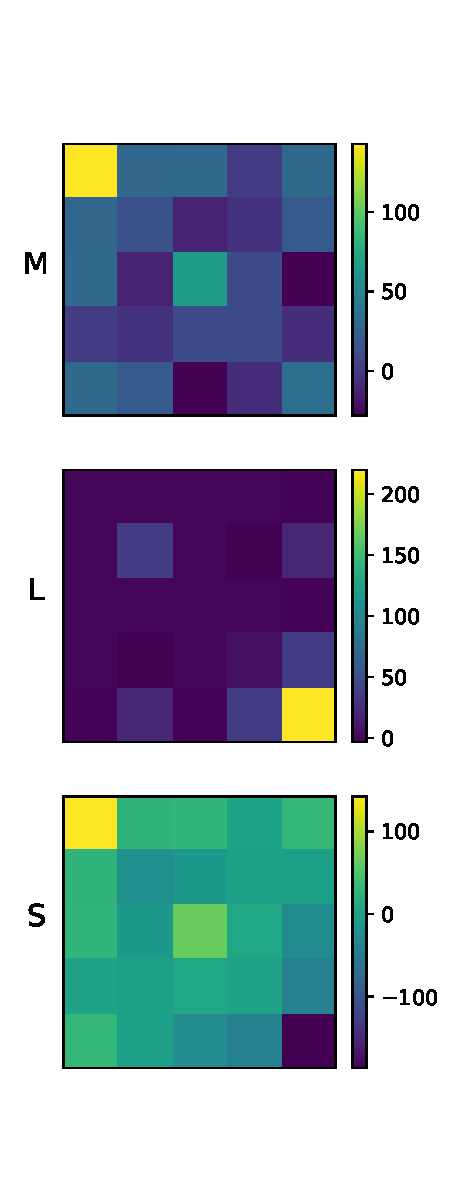
\includegraphics[width=0.48\textwidth]{fig/denise_output_finance.pdf}
	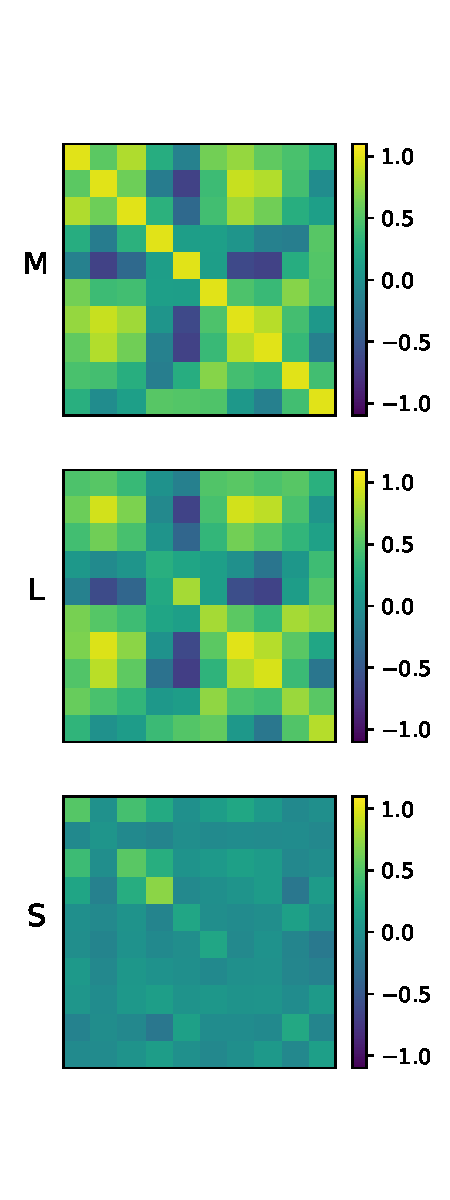
\includegraphics[width=0.48\textwidth]{fig/pcp_output_finance.pdf}
	\caption{Comparison of RPCA of the empirical $5\times 5$ covariance matrix of the prices of five share certificates (see main text) from the DAX 30. The left panel shows the resulting decomposition $M=L+S$ obtained from the neural network approach, while the right panel shows the results from PCP.}
	\label{fig:comp_finance}
\end{figure}


\subsection{Correlation matrix of personality features with PCP and Denise}
Here we compare the performance of the RPCA of our neural network approach and the benchmark PCP algorithm on 25 personality self report items obtained from approximately 2800 individuals. The studied 25 personality features are grouped in the five categories agreeableness, conscientiousness, extraversion, neuroticism, and opennness, see \href{https://www.personality-project.org/r/html/bfi.html}[personality-project]. The aim of PCA is to recover these five underlying putative factors from the data.

In this subsection we compare the performance of PCP and our neural network approach to obtain the RPCA-decomposition of the correlation matrix of the 25 personality features. The correlation is thereby defined as the normalized empirical covariance between the variables $x_i$
\[
M_{ij} = \text{Corr}(x_i,x_j) = \frac{\text{Cov}(x_i,x_j)}{\sqrt{\text{Var}(x_i) \text{Var}(x_i)}} \,.
\]
As in the previous subsection, we calculate the RPCA-decomposition $M=L + S$ by means of our neural network approach as well as by using the PCP method introduced in \ref{sec:pcpalgorithm}. The obtained low rank matrix $L$ and the sparse part $S$ containing corruptions of the input matrix are shown in Fig. \ref{fig:comp_psych}. The low-rank $k=10$ is determined by the PCP-algorithm, and subsequently used in the definition of the neural network.

As in the analysis of the financial data, the neural network decomposition exhibits very few strong outliers, which suppress the visual structure of the obtained matrices $L,S$ to some extend. As before, these outliers are not present in the PCP results. Hence, the PCP-method seems to function more stable than the network ansatz. \textcolor{red}{oreover, the sparsity of $S$ obtained from PCP is lower than from the neural network decomposition, indicating a performance advantage of PCP.}

\textcolor{red}{Distance between L,L S,S}

\textcolor{red}{In future we will use the decomposition to determine PC and to extract $k$ specific personality features..}

The comparison of both methods, in combination with the striking results reported in \cite{herrera2020denise}, may be explained by a sub-optimal choice of network-architecture (to few nodes per hidden layer) of our network. Another source of instability might result from the small training sets or not ideally chosen hyper-parameters such as batch-size. This will be analyzed in detail in future work.





\begin{figure}
	\centering
	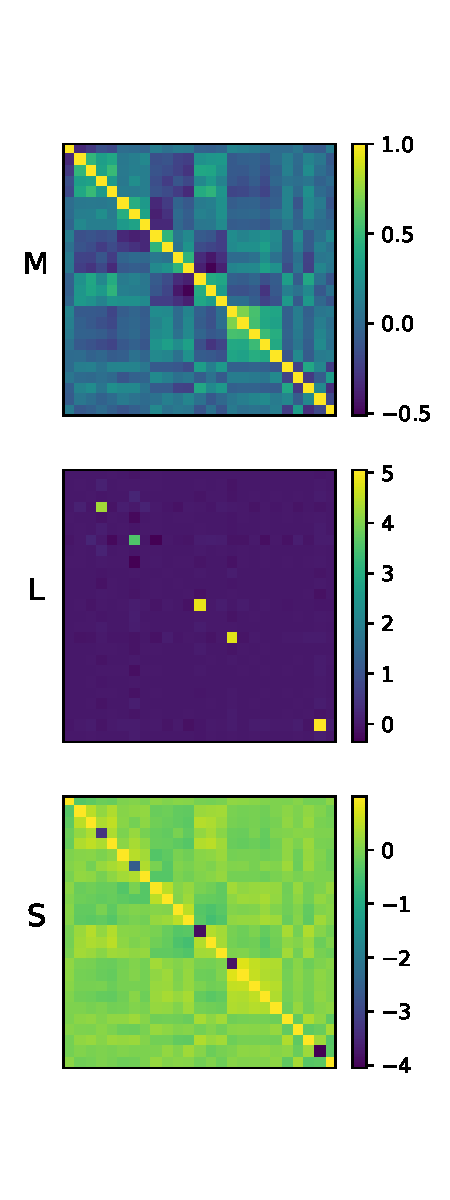
\includegraphics[width=0.48\textwidth]{fig/denise_output_psych.pdf}
	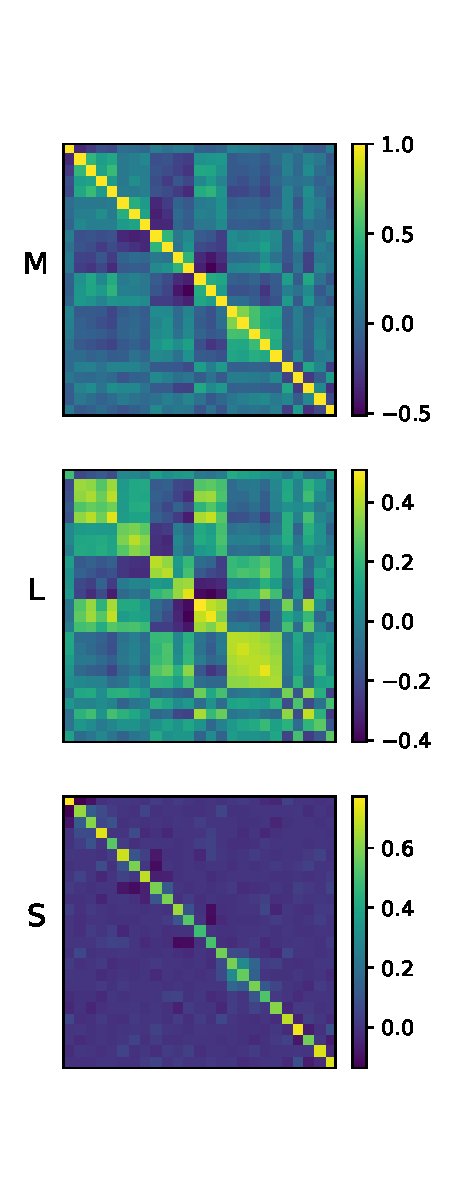
\includegraphics[width=0.48\textwidth]{fig/pcp_output_psych.pdf}
	\caption{Comparison of RPCA of the empirical $27\times 27$ covariance matrix of 27 personality features of roughly 2800 individuals (see main text). The left panel shows the resulting decomposition $M=L+S$ obtained from the neural network approach, while the right panel shows the results from PCP.}
	\label{fig:comp_psych}
\end{figure}








